\documentclass[11pt]{article}
\usepackage[T1]{fontenc}
\usepackage{lmodern,microtype}
\usepackage[margin=1in,headheight=14pt]{geometry}
\usepackage{amsmath,amssymb,amsthm,mathtools}
\usepackage{booktabs,longtable,array,enumitem}
\usepackage{xcolor,graphicx,fancyhdr}
\usepackage{tikz}
\usepackage{xurl}
\usetikzlibrary{arrows.meta,positioning}
\usepackage[colorlinks=true,linkcolor=navy,citecolor=teal,urlcolor=teal]{hyperref}
\definecolor{navy}{HTML}{18354A}
\definecolor{teal}{HTML}{007B83}
\definecolor{pale}{HTML}{EDF4F5}
\pagestyle{fancy}\fancyhf{}
\fancyhead[L]{\small Dual forest normalization}
\fancyhead[R]{\small ProveIt research continuation}
\fancyfoot[C]{\thepage}
\setlength{\emergencystretch}{2em}
\setlist{itemsep=3pt,topsep=5pt}
\newtheorem{theorem}{Theorem}[section]
\newtheorem{lemma}[theorem]{Lemma}
\newtheorem{proposition}[theorem]{Proposition}
\newtheorem{corollary}[theorem]{Corollary}
\theoremstyle{definition}
\newtheorem{definition}[theorem]{Definition}
\newtheorem{example}[theorem]{Example}
\newtheorem{remark}[theorem]{Remark}
\newcommand{\N}{\mathbb N}
\newcommand{\Z}{\mathbb Z}
\newcommand{\rootv}{\partial_*}
\newcommand{\supp}{\operatorname{supp}}
\newcommand{\rk}{\operatorname{rk}}
\newcommand{\poly}{\operatorname{poly}}
\newcommand{\st}{\operatorname{stop}}
\newcommand{\cl}{\operatorname{cl}}
\newcommand{\code}[1]{\texttt{\detokenize{#1}}}
\newcommand{\basecommit}{\nolinkurl{8cb7d9d25ac8cb64a9d147304e3441e98e94c7a4}}
\title{\color{navy}\bfseries Dual Forest Normalization and\newline Constrained Cancellation for\newline Compressed Unknot Hierarchies}
\author{Research continuation for Vladimir Reshetnikov's ProveIt project}
\date{12 October 2026}
\begin{document}
\maketitle
\begin{abstract}
The source-certified normal-cut pipeline in ProveIt rejects its finite
handlebody test whenever its complementary core contains a three-handle.
We remove this restriction by compiling the actual endpoint occurrences of
the core two-handles into a rooted dual graph.  A spanning tree specifies
geometric two-/three-handle cancellations.  For the native finite
torus-boundary source contract, the graph is always rooted, so all
three-handles can be removed in polynomial encoded time, independently of
normal-surface multiplicity.  The construction retains the exposed port
data needed by the existing boundary kernel and has an independent checker.

The choice of dual tree affects subsequent raw one-/two-handle cancellation.
We characterize successful choices as spanning trees meeting every stopping
set of an unsigned occurrence matrix.  This gives complete obstruction-guided
search, with a bound parameterized by the number of three-handles and the
sizes of the stopping witnesses encountered.  If each column containing
a unit entry is supported on at most two rows, the problem is polynomial: directed
reachability identifies mandatory strongly connected components, and a
graphic--partition matroid intersection chooses an independent transversal.
Negative certificates in this restricted problem are graphic rank defects.
We also prove that each original native column has at most three total
occurrences, with its odd entries forming a cycle in the dual graph.

We provide proofs, an additive native implementation, independent
certificate replay, finite search implementations, reproducible experiments,
and integration instructions.  Classical handle cancellation, matroid
intersection, and earlier stopping-set results are credited explicitly.
These results improve a supplied-cut terminal operator; they do not establish
a general quasi-polynomial unknot recognizer.
\end{abstract}
\tableofcontents
\newpage
\section{Research target, source state, and contribution}
\label{sec:scope}

\subsection{The particular obstruction addressed here}
The maintained algorithm has several mathematically distinct layers.
The complete recognizer can use exact invariant computations and other
certifying procedures.  The normal-surface research pipeline separately
constructs compressed cuts, their parallelity bundles, finite complementary
cores, ordered interfaces, and, when a sufficient criterion succeeds,
handlebody censuses.  A census records every component's genus and binary
multiplicity.  The latter pipeline supplies potential building blocks for
hierarchies, but it is not itself the complete unknot recognizer.

This work fixes one precise gap in that pipeline.  At the source revision
\basecommit\ \cite{ProveIt}, both the core certifier and the supplied-cut entry point
stop on a nonempty list \code{handles3}.  This is a conservative implementation
restriction, not a theorem that the corresponding manifolds are difficult.
The retained source charts already contain sufficient information to
remove these handles geometrically.  Our first contribution is to recover
that information, prove the reduction relative to the exposed interfaces,
and connect it to the existing independently checked boundary kernel.

The pinned files are in
\code{Topology/UnknotRecognition/fast/fastunknot/}; the principal entry point is
\code{normal_cut_handlebodies.py}.  The new branch reuses its already computed
parallelity packet.  It does not start a second parallelity discovery.
The new certificate is dispatched through
\code{normal-cut-handlebodies-v6}.  Earlier schemas remain supported.
The package includes the patch and a machine-readable source manifest.

\subsection{Why this is a continuation of the existing work}
We inspected the current implementation, the maintained synthesis, and the
ten archives in \code{docs/incoming} at the pinned revision.  Several tempting
ideas are already present there and are not claimed as discoveries here.
In particular:
\begin{itemize}
\item unsigned stopping sets and complete unit-column peeling are established
  by the incoming stopping-core and saturated-bundle reports;
\item cographic persistence uses chamber graphs to retain simultaneously
  nonseparating surfaces and accounts for causal resets;
\item modular Morse certificates verify supplied compressed matchings, with
  an explicit regular-geometry hypothesis;
\item genus budgets, sparse cut grammars, and native ordered interfaces already
  give several complementary size and attachment bounds.
\end{itemize}
None of those ten packages implements the native dual two-/three-handle
normalization developed below.  The combination of dual forest selection
with the stopping obstruction also poses a new optimization problem within
this development.  Its degree-two-column case leads to the polynomial
algorithm in Section~\ref{sec:sparse}.

Our novelty claims are deliberately local: a source-specific compiled
normalization and certificate interface, together with the stated
constrained-cancellation characterizations and algorithms.  We make no claim
that handle cancellation, spanning trees, or matroid intersection are new,
and no claim of an exhaustive priority search across all literature.

\subsection{Relationship to Lackenby's programme}
Lackenby's 2026 preprint \cite{Lackenby2026} presents a hierarchy algorithm
for essential boundary patterns and incompressibility.  Its
Proposition~9.1 bounds iterations by
\begin{equation}\label{eq:lackenby-iterations}
                 L(g+1)^L,
\end{equation}
where $L$ bounds hierarchy length and $g$ bounds surface pattern-complexity.
Its Section~9 explicitly separates this count from a full running-time
analysis.  The refined construction gives a linear bound on hierarchy
length in Proposition~10.2; the introduction leaves the intended speed-up
for further work.

There is also a distinction between two announced exponents.  Early Oxford
publicity uses $n^{O(\log n)}$ \cite{Oxford2021}.  The author's March 2021 slides
give $L=O((\log n)^2)$ and $g=O(n^2)$, resulting in
\begin{equation}\label{eq:announced}
       n^{O((\log n)^2)}=2^{O((\log n)^3)};
\end{equation}
the 2024 Tsinghua seminar description repeats this latter bound
\cite{LackenbySlides,Tsinghua2024}.  Both are quasi-polynomial, but they
are not identical.  We aim toward the general quasi-polynomial programme
without treating a local polynomial operator as a proof of either exponent.

Compressed cutting itself is established prior art.  Theorem~9.3 of
\cite{Lackenby2021} already gives a polynomial algorithm in triangulation
size and logarithmic surface weight, using Agol--Hass--Thurston orbit
methods \cite{AHT2006}.  Theorem~14.4 of \cite{Lackenby2026} gives the
uniform-handle version, including bundle type and attachment information.
Our contribution concerns an explicit subsequent native operator and its
certification.  It does not replace or re-prove those general existence
theorems.

\subsection{Statements proved and statements left open}
The main mathematical results are as follows.
\begin{enumerate}
\item The native dual graph has $O(t)$ vertices, edges, and incidence work.
  It is rooted for every admitted source and every admitted normal vector.
  Its spanning trees give geometric reductions of all core three-handles
  (Theorem~\ref{thm:native}).
\item This graph depends only on which source edge weights vanish.  A tree
  can therefore be reused throughout such a support stratum, including all
  positive scalar multiples (Corollary~\ref{cor:support}).
\item For a fixed lower spanning forest, successful dual trees are exactly
  the graphic bases that intersect every stopping set of the remaining
  unsigned occurrence matrix (Theorem~\ref{thm:transversal}).
\item Stopping witnesses give a complete parameterized search; insufficient
  graphic rank of a family of disjoint witnesses gives a rigorous obstruction
  (Theorem~\ref{thm:search} and Proposition~\ref{prop:packing}).
\item If every non-inert column has at most two incident rows, tree selection
  is polynomial and has explicit positive and negative certificates
  (Theorem~\ref{thm:degree-two}).  Every original native column has at most
  three total occurrences, isolating $(1,1,1)$ as the remaining native
  type (Proposition~\ref{prop:three}); its odd entries form a dual cycle
  (Proposition~\ref{prop:cycle}).
\end{enumerate}
The geometric scope is a supplied compressed cut with authenticated charts.
The exact search scope fixes the lower zero-/one-handle forest, allows the
specified dual-tree reduction, and then allows raw unsigned one-/two-handle
cancellation.  Failure of this restricted search proves no assertion that
the manifold is not a handlebody or that the original knot is nontrivial.
Arbitrary handle slides, changes of the lower forest, and hierarchy-wide
search remain outside that completeness theorem.

\section{Native dual normalization with retained interfaces}
\label{sec:geometry}

\subsection{Source contract and size parameters}
The native normal-surface validator supplies a connected finite triangulation
of a compact orientable three-manifold with one torus boundary.  Generalized
face pairings and self-identifications are permitted only when the validator's
manifold checks pass.  The normal vector is nonnegative and integral, satisfies
the matching equations and quadrilateral constraints, and belongs to the
existing source contract.  We do not weaken any of these checks.

Write $t$ for the number of tetrahedra, and $B$ for the largest bit length of
a coordinate or local edge weight, with $B\geq1$.  The source constructor
\code{normal_parallelity_geometry.py} partitions the cut into interval-bundle
regions and a finite complementary handle core.  Its $i$-handles are denoted
$H_i$.  The core has boundedly many local nonparallel regions per source
tetrahedron.  Crude bounds adequate here are
\begin{equation}\label{eq:handle-bounds}
 |H_0|\leq6t,\quad |H_1|\leq8t,\quad |H_2|\leq12t,
 \quad |H_3|\leq4t.
\end{equation}
Indeed, a tetrahedron contributes at most two central pieces and four
triangle tips; a paired face contributes at most four nonparallel regions;
each interior source edge contributes at most its two extreme gaps; and
three-handles correspond to interior source vertices.  The total number of
one-handle crossings in all source two-handle cycles is at most $12t$:
each local tetrahedral edge occurs in at most two extreme cycles.

The encoded core is thus small even when a normal coordinate is enormous.
Its three-handles retain their source vertex and incident link triangles.
Each two-handle retains its source edge, its gap rank, and its full cyclic
attaching chart.  These records are geometric incidence data; they are
strictly stronger than a signed cellular boundary matrix.

\subsection{The graph of actual belt-point occurrences}
\begin{definition}[Rooted dual graph]
Let $K$ be an authenticated finite three-dimensional handle core.  The
\emph{dual graph} $D$ has one vertex for each three-handle and a formal root
$\rootv$ for boundary not capped by a three-handle.  A two-handle is
$D^2\times I$ and has belt sphere $\{0\}\times\partial I$, consisting of
two points.  Its edge joins the labels of these two actual belt-point
occurrences.  A point in a three-handle's attaching sphere receives that
vertex label; an uncapped point receives $\rootv$.
\end{definition}

The root need not be a connected boundary component.  It is an algebraic
device joining all places at which cancellation can terminate.  Edges from
the root to itself and edges whose two ends are the same three-handle are
loops.  A loop has two occurrences, not zero.  This distinction prevents a
signed boundary coefficient from being mistaken for geometric cancellation.

For native cores, the graph is recovered without tracing an expanded normal
surface.  Fix an oriented source edge $e$, with original endpoints $u,v$ and
normal intersection weight $w_e$.
\begin{enumerate}
\item If $w_e=0$, there is a single core gap.  Its dual edge joins the labels
  of $u$ and $v$.
\item If $w_e>0$, there are two extreme core gaps.  Rank zero joins $u$ to
  $\rootv$, and rank $w_e$ joins $\rootv$ to $v$.
\end{enumerate}
An original boundary vertex is assigned $\rootv$.  The other $w_e-1$ gaps
belong to the parallelity structure and are never enumerated by this step.

\begin{lemma}[Correct source orientation]\label{lem:orientation}
The native source edge identifier is a representative of the signed
union-find class of local tetrahedral edges.  At that representative the
orientation parity is zero.  Thus decoding its local edge $(a,b)$ with
$a<b$ identifies the original endpoint of rank zero as $a$, and that of the
maximum rank as $b$, even when the two global endpoint vertices coincide.
\end{lemma}
\begin{proof}
The parity stored by the signed equivalence structure is the parity between
a local edge and its representative.  A representative is related to itself
with parity zero.  The source rank convention reverses ranks precisely when
this parity is one.  At the representative no reversal occurs, so the
claimed identification follows directly from the local edge parameter.
The global equality of vertex labels does not identify the two local endpoint
germs.
\end{proof}

One must not use an unordered endpoint cache to choose between the two
extreme ranks.  The implementation decodes the representative itself; the
independent checker reconstructs the same geometric fact separately.

\begin{lemma}[Root reachability]\label{lem:rooted}
For every native source and admissible normal vector, every vertex of $D$
is connected to $\rootv$.
\end{lemma}
\begin{proof}
The one-skeleton of the connected source triangulation is connected and
contains boundary vertices.  Identify all boundary vertices with one root.
Boundary edges then become root loops; removing them does not affect root
reachability.  Keep every interior source edge of zero normal weight.  Replace
each positive-weight interior edge by two root stubs, one from each of its
original endpoints to the root.  Replacing an edge in this way preserves root
reachability: any path that formerly used that edge can pass through the root
instead.  The resulting graph, after discarding irrelevant root loops, is
exactly the graph just compiled from extreme core gaps.  Its nonroot vertices
are exactly the interior source vertices, equivalently the core three-handles.
\end{proof}

\subsection{Geometric cancellation, including the relative assertion}
The following is a source-specific use of the classical handle cancellation
theorem: the attaching sphere of a $(k+1)$-handle must meet the belt sphere
of a $k$-handle transversely in one point \cite[Theorem~5.4]{Milnor1965}.
Here the belt sphere is zero-dimensional, so the compiled occurrence data
give the required geometric intersection directly.

\begin{lemma}[Rooted dual forest cancellation]\label{lem:dual-cancel}
Suppose every component of an authenticated dual graph meets its root.
For any spanning tree $T$ after the roots have been identified, there is a
sequence of geometric two-/three-handle cancellations deleting precisely
the two-handles labeled by $T$ and every three-handle.  The surviving
two-handles retain their attaching maps to the abstract zero-/one-handle
base.  No algebraic free reduction or two-handle slide is needed.

If a specified exposed boundary subcomplex has a collar disjoint from the
dual cancellation balls and tubes, the reduction preserves its labeled
embedding up to the relative boundary identification.
\end{lemma}
\begin{proof}
Orient the tree toward the root.  Choose a vertex adjacent to the already
exposed root region.  Its parent edge has one belt point in that
three-handle's attaching sphere and the other in exposed boundary.  The
classical cancellation criterion therefore applies.  Cancel the pair.
Other edges formerly incident with that three-handle now meet exposed
boundary.  On the dual graph this is precisely contraction of the selected
edge into the root.  Continue outward along the tree.  Each step removes one
three-handle; after $|H_3|$ steps the selected tree edges and all three-handles
have disappeared.

There is an elementary boundary-ball proof of each step, which also
establishes the relative assertion.  Write the cancelling two-handle as
$h_e=D^2\times[-1,1]$, with caps $D_e^\pm$.  Label it so that the
three-handle's attaching sphere $\Sigma$ contains $D_e^+$ and not
$D_e^-$.  Let $R$ contain all other handles.  Other three-handle spheres
miss both caps, so their attachments can be made before this pair.  Then
$\Delta=\overline{\Sigma\setminus D_e^+}$ is a disk in $\partial R$.
Together with the attaching annulus $A_e$ of $h_e$, it forms a disk
$E=\Delta\cup A_e$ in $\partial R$.  Meanwhile
$h_e\cup_{D_e^+}h_3$ is a three-ball $B$, and the original manifold is
$R\cup_E B$.  Adding a ball along a boundary disk adds only a collar.
The collar can be straightened relative to its boundary circle and to
every exposed patch in $R$ outside the interior of $E$.

The move alters the upper attachment boundary but does not introduce a
slide of any retained two-handle over another one.  Consequently the
attaching maps of all retained two-handles to the abstract lower base can
be kept as before.  This is a statement about the resulting handle
description.  It does not assert that a homeomorphism fixes every point of
the entire old lower submanifold.
\end{proof}

\begin{lemma}[Native exposed ports]\label{lem:ports}
The exposed core-facing ports of the native parallelity construction can be
retained by the reduction in Lemma~\ref{lem:dual-cancel}, with their incidence,
cyclic order, and side labels unchanged.
\end{lemma}
\begin{proof}
The native constructor places each core-facing port on an exposed region of
a zero-handle or a one-handle; its chart records \code{core_dimension} as
zero or one.  There are no ports in the interiors of core two- or
three-handles.  They are actual boundary patches of the complementary core,
not patches later covered by a three-handle.

In the boundary-ball proof of Lemma~\ref{lem:dual-cancel}, every port is
therefore contained in $R$.  It misses the interior of $E$: that interior
is an internal gluing region in $R\cup_E B$, not exposed boundary.
If a port edge meets $\partial E$, use the collar straightening fixed on
that circle.  The relative identification thus fixes all exposed port
patches.  Iterating this argument retains their product-chart boundary
identifications.  No port is deleted, reordered, or reattached, so its
signed word and its incidence with the unchanged abstract lower charts
are retained.
\end{proof}

This argument applies to the authenticated native ports.  A proposed future
boundary pattern that crosses the cancellation support must supply its own
transport.  The mere fact that a pattern has a small graph or an Euler
characteristic does not meet this requirement.

\begin{theorem}[Native top-handle normalization]\label{thm:native}
Given an authenticated native parallelity geometry, all core three-handles
can be removed by a certified geometric reduction.  Its reduced core and
retained exposed interfaces describe the same cut manifold with the same
parallelity attachments.  The reduction removes exactly $s=|H_3|$
two-handles, preserves Euler characteristic, and needs $O(t)$ graph records.

Graph compilation and a breadth-first tree use $O(t)$ arithmetic/label
operations.  Independent union-find verification uses
$O(t\alpha(t))$ label operations.  The arithmetic involves $B$-bit weights
and $O(\log(t+1))$-bit labels, so a deterministic array implementation has
polynomial bit cost, for example
\[
 O\bigl(tB+t\alpha(t)\log(t+1)\bigr)
\]
in a logarithmic-cost random-access model, after source authentication,
for the canonical bounded-size certificate.  The delivered producer uses
arrays and breadth-first search; replay uses separate arrays and union-find.
A multi-tape Turing implementation also has polynomial bit cost, without
asserting this exact random-access bound.  For arbitrary malformed input,
verification time additionally includes its actual encoded length; a huge
invalid identifier must be read before it can be rejected.
\end{theorem}
\begin{proof}
Apply Lemma~\ref{lem:rooted}, construct a tree, and use
Lemmas~\ref{lem:dual-cancel} and~\ref{lem:ports}.  A tree on $s+1$ vertices
has $s$ edges.  Removing equal numbers of two- and three-handles leaves the
alternating handle count unchanged.  The size bounds
\eqref{eq:handle-bounds} and the local edge-weight formula give the operation
bounds.  The independent checker needs only to reconstruct the selected
edge endpoints, reject cycles, and verify that all $s$ vertices reach the
root.  The list of selected original two-handle identifiers has
$O(s\log(t+1))$ bits; all retained charts can be shared or copied from the
authenticated source.
\end{proof}

\begin{corollary}[Support-stable normalization]\label{cor:support}
For a fixed source triangulation, the dual graph, using semantic labels
$(e,\text{zero})$, $(e,\text{left})$, and $(e,\text{right})$, depends only
on the set of edges with zero normal weight.  A selected dual tree is valid
throughout that stratum.  In particular it is valid for every positive
integer multiple of a supplied normal vector.
\end{corollary}
\begin{proof}
The two cases in the graph compiler use only $w_e=0$ or $w_e>0$.
The endpoint labels come from the source vertices and remain fixed.
Multiplication by a positive integer preserves every zero test.  Maximum
ranks are updated to the current $w_e$ when actual chart identifiers are
reconstructed.
\end{proof}

\begin{proposition}[Optimal initial deletion cost]\label{prop:max-tree}
Assign a nonnegative cost $c_e$ to every native two-handle, such as its
attaching-cycle length or its raw occurrence count after a fixed lower
forest.  A maximum-weight spanning tree minimizes the total cost of the
retained two-handles among all dual-tree normalizations.
\end{proposition}
\begin{proof}
For a tree $T$, the retained cost is
$\sum_{e\in E(D)}c_e-\sum_{e\in T}c_e$.  The first summand is constant.
Thus minimizing the retained cost is exactly the maximum spanning-tree
problem.
\end{proof}
This objective is inexpensive but does not guarantee subsequent raw
cancellability.  The next sections address that stricter question.

\section{Choosing the dual forest using raw cancellation obstructions}
\label{sec:forests}

\subsection{The restricted certificate class}
Fix a zero-/one-handle spanning forest $F$ in the core.  Contracting $F$
leaves one zero-handle in each component and some one-handles.  Every
two-handle has a geometric attaching cycle through their belt disks.  Let
\[
          A=(a_{rc})\in\N^{R\times C}
\]
be its unsigned occurrence matrix: $r$ labels a two-handle and $c$ a
surviving one-handle.  Signs and cancellations in the fundamental group are
not used.  Multiple geometric crossings contribute multiple occurrences.
One may saturate each count at two because only zero, one, and at least two
matter to the predicates below.

The same row set $R$ labels the edges of the rooted dual graph $D$.
When interface relations are included, give each row ineligible for top
cancellation an artificial root loop.  Such a row cannot be selected in
a tree; it still participates fully in every stopping test.
Choosing a dual spanning tree $T\subseteq R$ deletes its rows, by
Section~\ref{sec:geometry}.  We ask whether all remaining rows can be
removed by raw geometric one-/two-handle cancellation.  A raw pivot
$(r,c)$ requires $a_{rc}=1$ and has the unsigned update
\begin{equation}\label{eq:pivot}
       a'_{ih}=a_{ih}+a_{ic}a_{rh}
       \qquad (i\ne r,\ h\ne c),
\end{equation}
followed by deletion of $r$ and $c$.  This counts the crossings introduced
by pushing the other attaching bands through the cancelling pair.  It is
the conservative raw update used by the existing geometric certifier.
Saturating after each update preserves every future zero/one test.

\begin{definition}[Forest-compatible raw completion]
The pair $(D,A)$ is \emph{completable} if some spanning tree $T$ of $D$
leaves $A[R\setminus T,C]$ completely eliminable by pivots
\eqref{eq:pivot}.  The lower forest $F$ remains fixed throughout this
definition.
\end{definition}
This problem deliberately excludes normal isotopies that change occurrence
counts, arbitrary handle slides, and replacement of the lower forest.
Its positive answers are useful geometric certificates.  Its negative
answers have only the scope of this definition.

\subsection{Stopping sets and the exact raw criterion}
We recall the stopping-set theorem of the incoming stopping-core work
\cite{StoppingCores,SaturatedBundles}, including a proof because its invariant
is essential to the new search.

\begin{definition}[Stopping set]
A nonempty set $S\subseteq R$ is a stopping set when
\begin{equation}\label{eq:stopping}
          \sum_{r\in S}a_{rc}\ne1
          \quad\hbox{for every column }c.
\end{equation}
Equivalently every column has zero or at least two occurrences in $S$.
A \emph{unit-column peel} removes the unique row incident with a column
whose total is one.  The column can be removed as well: it has no other
occurrences, so this pivot creates no fill.
\end{definition}

\begin{lemma}[Canonical stopping residual]\label{lem:peeling}
Exhaustive unit-column peeling leaves the same row set regardless of
tie-breaking.  This set is the union of all stopping sets.  In particular
a row restriction is peelable exactly when it contains no stopping set,
and peelability is hereditary under deleting rows.
\end{lemma}
\begin{proof}
The union of stopping sets is stopping.  If a column had total one on the
union, its unique contributing row would belong to a constituent stopping
set on which that column also had total one, a contradiction.

A row in a stopping set cannot be peeled while the stopping set is intact,
because every column through that row has at least two occurrences within
the set.  Thus every stopping set survives every sequence of peels.  At
termination, if rows remain, their set is itself stopping.  It therefore
equals the union of all stopping sets and is independent of the order.
Finally a stopping subset of a smaller row restriction would also be a
stopping subset of the larger restriction, proving heredity.
\end{proof}

\begin{lemma}[Completeness for raw pivots]\label{lem:raw-complete}
All rows can be removed by arbitrary raw pivots \eqref{eq:pivot} if and only
if unit-column peeling removes all rows.
\end{lemma}
\begin{proof}
Peeling is a particular raw pivot sequence.  For the converse, suppose
$S$ is stopping and perform a raw pivot $(r,c)$.  If $r\notin S$, the
total $m=\sum_{i\in S}a_{ic}$ is zero or at least two.  In every remaining
column $h$, the new total is
\[
       \sum_{i\in S}a_{ih}+m a_{rh}.
\]
It is zero or at least two: a formerly zero total either stays zero or
increases by at least two, and a positive old total was already at least
two.  Thus $S$ remains stopping after removal of $c$.

If $r\in S$, then $m\geq2$ because $a_{rc}=1$.  Put
$S'=S\setminus\{r\}$.  The set $S'$ is nonempty; otherwise $S$ would
already have total one in column $c$.  In a remaining column its total is
\[
 \sum_{i\in S'}a_{ih}+(m-1)a_{rh}
       \ \geq\ \sum_{i\in S}a_{ih}.
\]
An old positive total was at least two, and an old zero total has all its
summands zero.  Hence $S'$ is stopping.  Inductively a nonempty stopping
set survives every pivot sequence, preventing complete elimination.
Lemma~\ref{lem:peeling} now proves the converse.
\end{proof}

The proof explains why signed exponent sums are inadequate.  A curve with
raw word $x x^{-1}x$ crosses the belt disk three times, even though its
group word freely reduces to $x$.  Treating these as one crossing silently
changes the permitted geometric move class.

\subsection{Spanning trees as transversals of obstructions}
\begin{theorem}[Forest--stopping-set equivalence]\label{thm:transversal}
Assume $D$ is connected after boundary roots are identified.  A spanning
tree $T$ is a successful forest-compatible raw completion if and only if
\begin{equation}\label{eq:hitting}
                   T\cap S\ne\varnothing
       \qquad\hbox{for every stopping set }S\subseteq R.
\end{equation}
Thus the problem is to choose a basis of a graphic matroid that is a
transversal of the stopping-set family.
\end{theorem}
\begin{proof}
If $T$ misses $S$, the same stopping set survives in $R\setminus T$, so
Lemma~\ref{lem:raw-complete} forbids completion.  Conversely, if the
restriction to $R\setminus T$ fails to peel, its nonempty canonical
residual is a stopping set missed by $T$.  Taking the contrapositive proves
the other direction.
\end{proof}

The family in \eqref{eq:hitting} can be exponentially large.  The theorem
is useful because a failed peel exposes a witness without listing the
whole family.  Moreover, peeling must not irrevocably reserve a row for
lower cancellation.  A row peeled during a partial search may still be
chosen later as a dual-tree edge.  Heredity makes this safe.

\subsection{Complete obstruction-guided search}
Maintain a selected forest $Q$ of dual edges.  Contract it in $D$ and remove
its rows from $A$.  Compute the stopping residual $K_Q$.  If it is empty,
extend $Q$ to any spanning tree of $D$ and finish.  Otherwise choose any
nonempty stopping subset $S\subseteq K_Q$, and branch on the edges
$e\in S$ that are not loops in $D/Q$.  The child adds $e$ to $Q$.
An inclusion-minimal stopping witness can be sought by successive row
removals and re-peeling, but minimality is not required for correctness.

\begin{theorem}[Complete forest search]\label{thm:search}
The preceding search is sound and complete for forest-compatible raw
completion.  Let $s=|V(D)|-1$ and let $w$ bound the sizes of the stopping
witnesses actually used.  Its branching depth is at most $s$, with at most
\begin{equation}\label{eq:search-nodes}
                     1+w+w^2+\cdots+w^s
\end{equation}
nodes.  If a node, including witness selection, costs $P(N)$ for encoded
input size $N$, the total cost is bounded by \eqref{eq:search-nodes} times
$P(N)$.  In particular it is $w^{O(s)}\poly(N)$ when $w\geq2$ and the
witness routine is polynomial; for $w=1$ it is $O((s+1)P(N))$.
\end{theorem}
\begin{proof}
A successful spanning-tree extension of $Q$ must meet any stopping witness
$S$ in a row not already in $Q$.  Every such edge is independent of $Q$,
so it appears in one of the stated branches.  Conversely each branch
retains independence and deletes exactly the rows that its chosen dual
edges cancel.  Thus branching neither omits a possible completion nor
creates a false one.

If $K_Q=\varnothing$, connectivity of $D$ ensures that the forest $Q$
extends to a spanning tree $T$.  The row set $R\setminus T$
is a subset of the already peelable set $R\setminus Q$.  Heredity proves
completion.  The final peel order should be recomputed or checked for
this actual $T$, rather than treating the earlier exploratory order as
an unverified certificate.

Each branch increases the forest rank by one.  A forest on $s+1$ vertices
has at most $s$ edges, proving the depth and node bounds.
\end{proof}

\begin{corollary}[A local quasi-polynomial regime]
If the source size and coordinate bit lengths are polynomial in a diagram
size $n$, and $s\log(w+1)=O((\log n)^k)$ for fixed $k$, this restricted
forest search has quasi-polynomial bit complexity.  The polynomial
degree-two-column algorithm in Section~\ref{sec:sparse} requires no small
bound on $s$.
\end{corollary}
This is a local certificate-class bound.  The source triangulation can have
linearly many interior vertices, and no bound on the total hierarchy work
follows from it alone.

\begin{proposition}[Packing obstruction]\label{prop:packing}
Let $Q$ be the currently selected forest, and let
$S_1,\ldots,S_p$ be pairwise disjoint nonempty stopping sets in
$R\setminus Q$.  A necessary condition for completion is
\begin{equation}\label{eq:packing}
       \rk_{D/Q}\left(\bigcup_{i=1}^p S_i\right)\geq p.
\end{equation}
For an edge set $X$, the rank is the number of vertices minus the number
of connected components of the graph with edge set $X$, including isolated
vertices and ignoring loops as rank contributions.
\end{proposition}
\begin{proof}
A completion must choose at least one edge from each $S_i$.  Disjointness
forces at least $p$ distinct chosen edges in their union.  These are part
of an independent forest in the contracted graph, so its rank is at
least $p$.
\end{proof}
In particular a stopping singleton is a mandatory tree edge.  If mandatory
edges form a cycle, no forest-compatible completion exists.  A stopping
witness whose every edge becomes a loop is the rank-zero case.  These
certificates use exact graph incidences and exact integer tests.

\subsection{Why tree choice matters, even for a ball}
\begin{example}[A geometric two-edge choice]\label{ex:choice}
Start with a solid torus, equipped with a fixed meridian belt disk for its
one-handle.  Choose two disjoint parallel primitive curves on its boundary.
Arrange the first to cross the belt disk once.  In the annulus complementary
to the first curve, a finger isotopy of the second adds a cancelling pair
of crossings, so the second crosses three times while remaining embedded
and parallel to the first.  Attach two two-handles along the curves and cap
one of the two resulting sphere boundaries with a three-handle.  Before
the cap the manifold is $S^2\times I$; after it the manifold is a ball.

The dual graph has one nonroot vertex and two parallel edges $a,b$ to the
root.  The raw occurrence matrix is
\[
                  A=\begin{pmatrix}1\\3\end{pmatrix}.
\]
Deleting $b$ leaves a raw singleton and succeeds.  Deleting $a$ leaves a
stopping singleton and fails.  Both choices are valid topological
two-/three-handle cancellations.  The difference lies entirely in the
subsequent restricted raw certificate.

If both primitive curves are given such finger pairs, the matrix becomes
$(3,3)^{\mathsf T}$.  Each row is a stopping singleton.  Their dual edges
have rank one, so \eqref{eq:packing} certifies impossibility in the raw
forest class.  The manifold is still a ball.  Thus even an exhaustive
negative answer in this class must remain inconclusive for handlebody
recognition.
\end{example}

This is a geometric existence example in a general handle structure.
Its actual column totals are four and six, respectively, so it is not
a native triangular-face core with the specified cocore.  Capping counts
preserves the finite cancellation decision, but does not authenticate a
native realization.  The example establishes that forest choice can
matter geometrically; the source tests provide the separate native evidence.

\begin{example}[Peelable row sets are not a matroid]\label{ex:nonmatroid}
Consider rows
\[
 r_0=(0,0,1),\quad r_1=(0,1,1),\quad
 r_2=(1,1,0),\quad r_3=(1,1,1).
\]
The row sets $X=\{r_2,r_3\}$ and $Y=\{r_0,r_1,r_2\}$ both peel and
$|X|<|Y|$.  But the column totals of $X\cup\{r_0\}$ are $(2,2,2)$,
and those of $X\cup\{r_1\}$ are $(2,3,2)$.  Both enlarged sets are
stopping.  The augmentation axiom therefore fails.  One cannot solve the
general problem merely by declaring peelable row sets to be a second
matroid.  The next section obtains a matroid formulation from a genuine
structural restriction on column support.
\end{example}

\section{A polynomial theorem for sparse active columns}
\label{sec:sparse}

\subsection{Replacing peeling by directed reachability}
Call a column \emph{inert} if none of its entries is one.  Every row
restriction still has no unit entry in that column, so it can never supply
a unit-column pivot.  Its sums on stopping sets can never equal one.
It may therefore be ignored for this decision, while its one-handle is
retained in the topological count.  Assume every non-inert column of $A$
has at most two nonzero rows.  Counts can still be arbitrarily large;
they are not assumed to be zero/one.  Define a
directed graph $P$ on the row set $R$ as follows.
\begin{itemize}
\item A column supported only on $r$ with $a_{rc}=1$ makes $r$ an initial
  seed.  A singleton entry of two or more makes no seed.
\item For a column supported on $\{u,v\}$, add an arc $v\to u$ if
  $a_{uc}=1$, and an arc $u\to v$ if $a_{vc}=1$.
\item Inert columns, including zero columns, make no contribution.
  Multiple arcs can be merged.
\end{itemize}
The direction records an implication: deleting the tail makes the head a
unit-column row.  Let $Z$ be the set of initial seeds.

\begin{lemma}[Exact reachability model]\label{lem:reachability}
For any set $Q$ of rows deleted by top cancellations, the union of $Q$
and all rows subsequently removed by unit-column peeling is exactly the
set reachable in $P$ from $Z\cup Q$.
\end{lemma}
\begin{proof}
Every initial seed can peel.  If an arc $v\to u$ comes from a column,
then that column has exactly one occurrence on $u$ and no possible other
row except $v$.  Once $v$ is deleted, $u$ can peel.  Induction on path
length therefore shows that every reachable row is removed.  The
certifying column cannot have been used and removed while its head row
was still live: at a unit-column pivot it had no other live owner.

Conversely, a row peeled at any step is certified either by a singleton
unit column, making it an initial seed, or by a two-row column whose other
row has already been removed.  In the latter case the corresponding
directed arc gives a reachability step.  Induction on the peel sequence
proves the reverse inclusion.
\end{proof}

Let the strongly connected components of $P$ be contracted into its
acyclic condensation graph.  Call a component a \emph{mandatory component}
if it is a source of this condensation graph and contains no initial seed.
List these components as $S_1,\ldots,S_q$.

\begin{lemma}[The only mandatory groups]\label{lem:mandatory}
Deleting $Q$ allows complete peeling if and only if
\[
                        Q\cap S_i\ne\varnothing
                           \quad(1\leq i\leq q).
\]
The $S_i$ are pairwise disjoint stopping sets.
\end{lemma}
\begin{proof}
A source component with no seed cannot be reached from another component.
It therefore needs a row of $Q$.  Conversely every component of a finite
acyclic graph is reachable from some source.  If each source either contains
a seed or is met by $Q$, all rows are reachable, and
Lemma~\ref{lem:reachability} applies.

To see that a mandatory component is stopping, consider a column having
an occurrence on a row of $S_i$.  If it has only one row and count one,
that row would be a seed.  If it has exactly one row in $S_i$, another row
outside $S_i$, and count one on the inside row, it would give an incoming
arc to the source component.  Both cases are impossible.  If both rows
are inside, the total is at least two; if the only inside count is larger
than one, the same is true.  An inert column can never sum to one.
Hence every column has zero or at least two
occurrences on $S_i$.
\end{proof}

\subsection{Independent representatives in a graph}
Each mandatory component is a set of row labels and therefore a set of
edges of $D$, with ineligible rows represented by root loops.  The groups
are disjoint.  We need one edge from each group,
with all chosen edges independent in the graphic matroid.  Such a partial
forest can be extended to a spanning tree, and any spanning tree meeting
the groups contains such a partial forest.

For completeness we state and prove the independent-representatives
criterion, a classical result of Rado \cite{Rado1942}.

\begin{lemma}[Rado's rank criterion]\label{lem:rado}
Let $M$ be a matroid and $S_1,\ldots,S_q$ finite subsets of its ground set.
There exist distinct representatives $e_i\in S_i$ forming an independent
set if and only if
\begin{equation}\label{eq:rado}
       \rk_M\left(\bigcup_{i\in J}S_i\right)\geq |J|
       \qquad\text{for every }J\subseteq\{1,\ldots,q\}.
\end{equation}
\end{lemma}
\begin{proof}
Necessity follows by restricting an independent representative set to $J$.
The case $q=0$ is empty.  For sufficiency induct on $q$.  The case $q=1$
says that $S_1$ contains
a nonloop, which follows from its positive rank.

Suppose a nonempty proper subfamily $J$ is tight in \eqref{eq:rado}.
By induction choose independent representatives $B$ for $J$.  They have
cardinality and rank $|J|$, so they span $U_J=\bigcup_{i\in J}S_i$.
For a set $K$ of remaining groups, contraction by $B$ gives
\[
 \rk_{M/B}(U_K)
   =\rk_M(U_K\cup B)-|J|
   =\rk_M(U_K\cup U_J)-|J|
   \geq |K|.
\]
Apply induction in the contracted matroid to the remaining groups.  Their
representatives together with $B$ give the required independent set.

If there is no nonempty proper tight subfamily, every such subfamily has
rank at least its size plus one.  Choose any nonloop $e\in S_q$.
For a nonempty set $K\subseteq\{1,\ldots,q-1\}$,
\[
            \rk_{M/e}(U_K)\geq\rk_M(U_K)-1\geq |K|.
\]
Induction after contracting $e$ supplies the remaining representatives;
adjoining $e$ finishes the proof.  The contraction treats $e$ as absent
from the remaining ground set, so the representatives are distinct.
\end{proof}

\begin{theorem}[Polynomial forest choice in the two-row regime]
\label{thm:degree-two}
Suppose $D$ is a connected rooted multigraph, and every non-inert column
of $A$ has at most two nonzero rows.  Compute the mandatory components
$S_1,\ldots,S_q$ of $P$.  Then the following are equivalent:
\begin{enumerate}
\item $(D,A)$ has a forest-compatible raw completion;
\item the groups $S_i$ have an independent system of representative edges
  in the graphic matroid of $D$;
\item for every set $J$ of mandatory groups,
\begin{equation}\label{eq:graphic-rado}
             \rk_D\left(\bigcup_{i\in J}S_i\right)\geq |J|.
\end{equation}
\end{enumerate}
These conditions can be decided in polynomial time.  A positive certificate
is a spanning tree with an explicit complete peel order.  A negative
certificate is a subfamily $J$ violating \eqref{eq:graphic-rado}, together
with the mandatory-component data, which can be recomputed independently.
\end{theorem}
\begin{proof}
Lemma~\ref{lem:mandatory} reduces completion to choosing a spanning tree
meeting each mandatory group.  Such a tree contains independent
representatives.  Conversely an independent representative set extends
to a spanning tree, which meets every group and therefore succeeds.
Lemma~\ref{lem:rado} proves the equivalence with the rank inequalities.

For the algorithmic assertion, restrict the ground set to the union of
the groups.  Intersect the graphic matroid with the partition matroid
allowing at most one edge from each group.  A common independent set
of size $q$ gives the representatives.  Matroid intersection has a
polynomial augmenting-path algorithm with independence oracles
\cite{Edmonds1979}.  Here the oracles are elementary: a
disjoint-set forest detects graphic cycles, and color counts test the
partition condition.  The residual exchange graph of a failed maximum
intersection produces a rank defect; equivalently the matroid-intersection
min--max theorem and Lemma~\ref{lem:rado} supply the subfamily $J$.
The delivered implementation extracts such a witness and its checker
verifies the inequality directly, without trusting an optimality assertion.
\end{proof}

\subsection{Explicit algorithm and complexity scope}
The algorithm first scans columns to detect the unsupported case of an
active column with more than two incident rows.  It then computes seeds,
arcs, strongly connected
components, and mandatory groups.  These steps take linear time in the
matrix incidence size, with standard adjacency-list graph algorithms.

Starting from the empty common independent set, the matroid-intersection
algorithm builds an exchange graph.  Its vertices are candidate edges.
Arcs encode exchanges that preserve one of the two matroids, and endpoints
encode single-element additions that preserve the other.  A shortest
augmenting path toggles membership and increases the common independent
set by one.  If no path exists, the reachable set yields the min--max
certificate.  There are at most $q\leq|R|$ augmentations.  Even a conservative
implementation using $O(|R|^2)$ oracle calls per augmentation and rebuilding
a graphic oracle in $O(|R|+|V(D)|)$ operations is polynomial:
\[
 O\bigl(I+|R|^3(|R|+|V(D)|)\bigr),
\]
where $I$ is the occurrence-input size.  No enumeration of all subsets $J$
in \eqref{eq:graphic-rado} is required.  The implementation and measured
operation counts are documented in Sections~\ref{sec:implementation}
and~\ref{sec:experiments}.

The column restriction is a geometric crossing restriction in an
authenticated core, not a bound on algebraic rank or on the number of
vertices of $D$.  Large counts on either of the two rows are permitted.
For example, an abstract solver input column $(1,2^{1000})^{\mathsf T}$
contributes just the arc
from the second row to the first.  A column with entries $(2,2,2)$ is
inert and harmless for the restriction.  A column with entries $(1,1,1)$
is outside the theorem.  These large-count examples concern the generalized
finite solver, not the original native columns bounded below.

\subsection{Why shortest augmentation works, and where the obstruction comes from}
Here is a self-contained justification for the specialized exchange step.
Restrict to the union $G$ of the mandatory groups and maintain a rainbow
forest $F$.  The exchange graph has sources $e\notin F$ for which $F+e$
is a forest and targets $e\notin F$ of an unrepresented group.  For
$f\in F$ and $e\notin F$ it has arcs
\[
 f\longrightarrow e\quad\hbox{if }F-f+e\hbox{ is a forest},\qquad
 e\longrightarrow f\quad\hbox{if }F-f+e\hbox{ is rainbow}.
\]
Take a shortest source-to-target path
$e_0,f_1,e_1,\ldots,f_\ell,e_\ell$.  None of its intermediate outside
vertices is a target, so $e_{i-1}$ has the group of $f_i$, whereas
$e_\ell$ has a new group.  The symmetric difference is therefore rainbow
and has $|F|+1$ edges.

For graphic independence, represent edges by vertex-incidence vectors
over $\mathbb F_2$.  The forest vectors are independent.  The source
$e_0$ is outside their span.  Every later $e_i$ is not a source, since
otherwise its suffix would shorten the path.  It therefore has a unique
fundamental cycle in $F$.  Its expansion in the forest basis has
coefficient one at $f_i$ and coefficient zero at each $f_j$ with $j<i$;
a nonzero earlier coefficient would supply the shortcut $f_j\to e_i$.
Modulo $F\setminus\{f_1,\ldots,f_\ell\}$ these expansions form a
triangular matrix with unit diagonal.  They are independent, and adding
$e_0$, outside the original span, preserves independence.  The augmented
set is a larger rainbow forest.

If no target is reachable, let $W$ be the reachable set of edge labels.
Every group appearing in $W$ is represented by an edge of $F\cap W$:
an unrepresented reachable group would give a target, and an outside
edge in a represented group has an arc to that group's selected edge.
Thus exactly $|F\cap W|$ groups appear in $W$.  Each outside edge not
in $W$ is spanned by $F\setminus W$: it is not a source, and its
fundamental cycle has no reachable selected edge, which would give an
incoming exchange arc.  Hence
\[
                   \rk_D(G\setminus W)=|F\setminus W|.
\]
Let $J$ consist of the groups with no edge in $W$.  If $|F|<q$, then
\[
 \rk_D\left(\bigcup_{j\in J}S_j\right)
 \leq |F\setminus W|
 =|F|-|F\cap W|<q-|F\cap W|=|J|.
\]
This supplies the claimed negative certificate directly.  The checker
only needs the stopping sets and the rank inequality, not the internal
exchange graph.

\subsection{A geometric bound isolating the remaining native case}
\begin{proposition}[Three occurrences per native cocore]\label{prop:three}
For the unsigned matrix of original native core two-handles against
native one-handle cocores,
\[
                         \sum_r a_{rc}\leq3
                    \qquad\hbox{for every column }c.
\]
The same holds after contraction of a fixed lower zero-/one-handle forest
and any dual-tree row deletion.  It is not asserted after adding boundary
relations or performing later handle slides.
\end{proposition}
\begin{proof}
Work in one abstract triangular source face before quotient identifications.
Its disjoint normal arcs have endpoints on distinct local sides.  Every
complementary disk region meets each of the three sides in at most one
gap.  This follows inductively: an additional arc splits one region,
divides its intervals on the two endpoint sides between the children,
and leaves each other side interval wholly in at most one child.
Initially the assertion holds for the uncut triangle.

The cocore of a native one-handle is one such face region.  Each geometric
traversal by a core two-handle corresponds to an actual boundary-gap
occurrence on that cocore, of which there are at most three.  Different
occurrences remain counted even if quotient identifications give them
the same global edge or handle label.  Removing parallelity two-handles
can only decrease the count.  Lower forest contraction deletes its
columns and introduces no crossings of retained cocores.  Dual-tree
normalization deletes rows while retaining their attaching charts.
\end{proof}

Consequently, up to permutation, every nonzero native column has
positive-entry multiset
\[
        (1),\ (2),\ (3),\ (1,1),\ (1,2),\ \hbox{or }(1,1,1).
\]
The last shape is the only one outside Theorem~\ref{thm:degree-two}.
For its three rows $u,v,w$, peeling gives the two-premise implications
$\{u,v\}\to w$, $\{u,w\}\to v$, and $\{v,w\}\to u$.
This is a precise point at which ordinary directed reachability ceases
to suffice.

\begin{proposition}[Parity compatibility with the dual graph]
\label{prop:cycle}
Use the actual unsaturated source counts in this statement.  Before top
cancellations, the dual edges whose entries in a fixed source column are
odd form an even-degree subgraph of $D$.  The same statement
holds for the retained rows in $D/Q$ after contracting a selected dual
forest $Q$.
\end{proposition}
\begin{proof}
Work over $\mathbb F_2$.  In the handle chain complex, the boundary of
a three-handle records the actual cap incidences of its two-handles
modulo two.  Thus $\partial_3$ is the incidence matrix of $D$ with the
formal root row omitted, transposed to the handle-boundary convention.
The corresponding row of $\partial_2$ is the unsigned source column
modulo two.  The identity $\partial_2\partial_3=0$ implies even degree
at each three-handle vertex.  Loops contribute twice.  The root also
has even degree, since the sum of all graph degrees is even.  Contraction
of a nonloop combines its endpoint parity equations and deletes that
edge; an even subgraph remains even in the contracted multigraph.
Iterate along $Q$.
\end{proof}

A native $(1,1,1)$ column is therefore a three-edge mod-two cycle:
a triangle, a parallel pair together with a loop, or three loops.
A singleton odd entry must label a dual loop.  These are necessary
geometric compatibility conditions, not a realization theorem for arbitrary
matrices.  The nonmatroid example in Section~\ref{sec:forests} already
has column totals $(2,3,3)$.  It can also satisfy the parity condition:
make $r_0,r_2,r_3$ three parallel root-to-vertex edges and $r_1$ a loop.
Its three columns are then even subgraphs.  Thus neither of these two
necessary conditions restores the matroid exchange axiom.  No native
triangulated realization of that example is claimed.

\subsection{The boundary between polynomial and general search}
Theorem~\ref{thm:degree-two} does not establish an intrinsic complexity
dichotomy for all handle structures.  We do not prove the unrestricted
problem NP-hard, and an improved algorithm may exist for other classes.
The exact obstruction-guided procedure remains available when the column
restriction fails.  Its canonical residual and graphic contraction can
also expose a smaller two-row instance later in the search.

A practical implementation can therefore use the polynomial solver first,
then use the general search with an explicit budget.  Positive output
always carries a tree and checked peel order.  Exhaustion under a budget
must produce an inconclusive status; it must not be confused with a
negative rank certificate or an exhaustively checked search tree.

\section{Implementation, certificates, and integration}
\label{sec:implementation}

\subsection{A small extension to the native entry point}
The production-facing change is deliberately confined to a supplied-cut
operation.  Four new modules implement geometric graph compilation, its
independent replay, the completed boundary-kernel branch, and its replay.
Two existing entry points acquire a dispatch to the new branch.  The graph
and reduction routines receive the authenticated geometry that the caller
has already constructed.  Consequently their introduction does not repeat
the weighted-orbit discovery that dominates some cuts.

The producer follows this sequence:
\begin{enumerate}
\item Compile the actual cap endpoints of every source core two-handle.
  Maintain a dense array of source vertex flags; exposed flags receive
  the root label.  No array is indexed by a normal coordinate value.
\item Find a rooted breadth-first tree.  Delete its two-handles and all
  three-handles, preserving the surviving two-handle order and assigning
  consecutive reduced identifiers.  Keep the lower charts, ports, and
  source coordinates intact.
\item Construct the existing ordered parallelity boundary skeleton, using
  the remainder of the caller's orbit budget.  Run the existing finite
  boundary kernel on the reduced geometry and that skeleton.
\item If the kernel completes, return its exact component census and, when
  requested, the composite certificate.  Otherwise return an inconclusive
  result with the recorded stage and reason.
\end{enumerate}
The shipped native producer uses a deterministic breadth-first tree.  The
more sophisticated forest solvers are delivered as separate research
modules and are used in the matrix audit.  They are not silently inserted
into the production entry point.  On the ten affected corpus cuts, exhaustive
fixed-kernel analysis finds no additional positive census beyond the seven
obtained by this simpler native branch.

\subsection{The composite certificate and trust boundary}
The new outer schema is \code{normal-cut-handlebodies-v6}.  Its exact
fields are \code{schema}, \code{parallelity}, \code{boundary},
\code{dual}, \code{kernel}, and \code{census}.  The two source packets
are the existing normal-parallelity and ordered-boundary certificates.
The new inner schema is \code{source-core-dual-forest-v1}, with just
\code{schema} and \code{forest}; the latter is a list of original
two-handle identifiers.

The independent outer checker first authenticates both source packets from
the supplied triangulation and normal vector.  It then reconstructs cap
endpoints and checks the supplied tree by union--find.  It requires exactly
$s$ distinct, valid, acyclic edges and verifies connection to the root.
It constructs the retained chart separately, replays the existing boundary
kernel, and compares the claimed census with the reconstructed one.
The independent dual checker imports no graph compiler or forest producer.
It uses its own endpoint table, a different root label, and independent
connectivity bookkeeping.  Sharing the mathematical endpoint convention
is necessary; sharing a producer's unchecked graph would not be sufficient.

The inner checker is intentionally a checker for \emph{authenticated}
geometry, not a substitute for the source validator.  Calling it directly
on an arbitrary dictionary does not authenticate a three-manifold.  This
precondition is documented in the modules and is enforced by the outer
entry point.  The contract excludes false inferences from an algebraic
incidence matrix: a coefficient of $\pm1$ is not accepted as a geometric
two-/three-handle cancellation without the actual cap occurrences.

Native source integers use the repository's exact integer codec.  Large
binary multiplicities survive replay and census comparison without a
machine-word truncation.  The tree itself uses only $O(t)$ source labels.
Normal weights occur only in endpoint arithmetic and in the already
existing source and bundle packets.  The statement that the new stage is
polynomial in encoded size is not a statement that every previous stage's
implementation has the same tight bound.

\subsection{Failure and resource semantics}
Successful native output is \code{COMPLETE}; all uncompleted native paths
are \code{INCONCLUSIVE}.  In particular, inability to root a supplied dual
graph is conservative even though Theorem~\ref{thm:native} rules it out
under the native contract.  A stalled boundary kernel is also conservative.
Neither status asserts that the source knot is nontrivial.

The callback used by the existing pipeline is propagated through graph
construction, adjacency traversal, boundary processing, and replay.
The outer verifier's \code{max_operations} parameter bounds the existing
orbit-proof operation records; it is not a universal bound on every Python
instruction or on arbitrary malformed input length.  The callback remains
the surrounding cancellation mechanism.  A hard total verification budget
would need a separate, consistently charged policy across all imported
checkers.  The tests preserve the current semantics rather than inventing
an incompatible interpretation for this one branch.

The finite graph/matrix solvers use \code{SUCCESS}, \code{NO_FOREST},
and \code{INCONCLUSIVE}.  Their negative statement has a different and
strictly specified meaning: no compatible tree completes raw cancellation
in that supplied model.  They can certify this by a disconnected graph
cut, a disjoint stopping-set rank defect, or a complete obstruction search
tree.  A disconnected finite input is useful for checker testing; it cannot
arise from the admitted native source graph.  Work or node exhaustion, and
the general Python producer's interpreter recursion limit, give only
\code{INCONCLUSIVE}.  The complete mathematical search theorem refers to
the finite procedure with sufficient resources.

\subsection{The separate finite graph/matrix implementation}
The source object has an integer vertex count, an integer column namespace,
one sparse occurrence row per two-handle, and one graph edge or \code{null}
per row.  Vertex zero is the root.  A \code{null} row is not eligible for
top cancellation; this covers the extra annular relations in the boundary
kernel.  Equivalently, the theory may give every such row an artificial
root loop.  This convention allows the same stopping criterion to include
both deletable source relations and nondeletable interface relations.

Counts are replaced by their values capped at two.  Sparse dictionaries
retain only named columns, so a very large binary column namespace does
not allocate that many entries.  Input validation rejects duplicate
incidences and malformed labels.  The graph checker also detects an omitted
isolated vertex without allocating a declared, potentially enormous
namespace.  These details keep validation tied to the supplied encoding.

The polynomial producer computes initial unit seeds and directed arcs,
then the source strongly connected components.  A shortest-path exchange
algorithm constructs a rainbow graphic forest.  The general producer
computes the stopping core, optionally shrinks a witness to inclusion
minimality, contracts a chosen graph edge, and branches only on eligible
nonloops.  Singleton choices are forced.  Every positive result includes
the final spanning tree and a peel order on the immutable source rows.
The verifier checks each advertised unit-column pivot against those rows,
without running the producer's peeling queue or exchange search.

For a rank obstruction the checker verifies that the listed row groups
are disjoint, nonempty stopping sets; computes the rank of their eligible
edge union; and checks that this rank is smaller than the number of groups.
It does not need to trust that the producer identified strongly connected
components correctly.  For a negative search tree it checks every node's
stopping set and exact coverage of the eligible branches, including the
accumulated forest contractions.  This distinction between discovering
and checking a witness is central to the implementation.

\subsection{Verification strategy}
The native focused tests cover the source orientation convention, ordinary
and loop edges, self-identifications, multiple interior vertices, geometric
port retention, exact Euler characteristic, source and certificate
mutations, older-schema dispatch, resource callbacks, one-sided normal
surfaces, and very large binary multiplicities.  An independent cap oracle
walks source local incidences on all 106 corpus cuts.  Producer-disabled
tests ensure that replay does not call the new discovery routines.

The finite focused tests include true augmenting paths of length three,
rank defects requiring a proper subfamily of source components, exhaustive
negative proof-tree coverage, loops and parallel edges, ineligible rows,
nonunit counts, huge sparse namespaces, and adversarial certificate
mutations.  The larger oracle audit separately enumerates spanning trees
and nonempty stopping subsets on small cases.  This tests both positive
and negative claims against a structurally different decision procedure.

These are executable regression and cross-checking tests, not a formal
proof assistant development.  The manuscript supplies the mathematical
proofs, and the checkers reduce the executable trust surface.  Regina
\cite{Regina} supplies a further, independently implemented topological
comparison for the new native positive censuses.

\subsection{Integration boundaries}
The package targets the exact source revision \basecommit.  Apply its
patch to that revision, run the focused tests and source replay, and then
rebase through the current entry points if the repository has advanced.
The small dispatch changes should be reviewed especially carefully against
newer certificate schemas or budget semantics.  The patch does not revise
the full recognizer's verdict logic, widen the native source validator,
or assert completeness of the boundary kernel.

The standalone forest module is ready for experimentation but remains a
separate integration decision.  A future production importer must bind
its matrix to authenticated geometric words and label every nondeletable
relation correctly.  The matrix audit included here demonstrates that
binding for the current fixed boundary kernel; it does not justify
reusing a cached matrix after an unrecorded change of lower forest,
interface attachment, or handle slide.

\section{Experiments and what they establish}
\label{sec:experiments}

\subsection{Pinned corpus comparison}
The baseline is the supplied-cut entry point at \basecommit, loaded from
that exact Git object.  Its dependencies are held at the same revision.
The corpus is the 106-case \code{marked_parallelity_research/corpus.json}.
Its SHA-256 digest and the baseline entry-point digest are recorded in
\code{results/native/native_audit.json}.  Every result records a case label,
statuses, timing scope, census when present, and certificate information.

\begin{table}[htbp]
\centering
\caption{Native supplied-cut census coverage at the pinned revision.}
\label{tab:coverage}
\begin{tabular}{lrr}
\toprule
Outcome & Baseline & With dual normalization\\
\midrule
Complete censuses & 85 & 92\\
Inconclusive cuts & 21 & 14\\
Earlier complete censuses preserved & -- & 85\\
Successful independent certificate replays & -- & 92\\
New censuses agreeing with Regina & -- & 7\\
\bottomrule
\end{tabular}
\end{table}

The coverage rises from $80.19\%$ to $86.79\%$.  Seven of the 21
previously inconclusive cuts become complete, reducing that count by one
third.  This is a measured coverage improvement on supplied cuts.  It is
not a measured speed-up of the end-to-end knot recognizer, and a previous
inconclusive return is not a valid fast baseline for a newly completed
query.  The README's older success count is stale; the comparison uses
the measured 85 rather than that prose count.

\begin{table}[htbp]
\centering\small
\caption{All seven newly certified cuts.  The notation $g^m$ means
$m$ components of genus $g$, not exponentiation.}
\label{tab:new-cuts}
\begin{tabular}{p{0.69\textwidth}l}
\toprule
Corpus label & Genus census\\
\midrule
\code{pilot/interior_1_2/0} & $1^2$\\
\code{pilot/interior_2_3/0} & $1^2$\\
\code{pilot/interior_3_5/0} & $1^1$\\
\code{pilot/finite_trefoil_interior/0} & $2^1$\\
\code{interior_1_2/mixed} & $0^2$\\
\code{interior_3_5/mixed} & $0^2$\\
\code{finite_figureEight_interior/mixed} & $0^1,2^2$\\
\bottomrule
\end{tabular}
\end{table}

The package retains the seven full source/certificate packets.  The audit's
sorted-key JSON encodings of the seven composite certificates alone range
from 11,631 to 1,069,420 bytes.  The
last, larger certificate mainly reflects existing source and boundary
proofs, not a large dual tree.  All seven affected native trees have one
edge in this corpus.  Separate subdivision fixtures exercise many
three-handles, so the tests of the graph stage are not confined to
one-edge cancellation.

\subsection{Which matrices need more than the polynomial theorem?}
The matrix audit first fixes the native lower zero-/one-handle spanning
forest and reads the original source two-handle cycles.  Of the 106
matrices, 12 have maximum column support zero, seven have maximum support
one, 62 have maximum support two, and 25 have maximum support three.
Thus 81 of 106 satisfy the two-row condition before adding interface
relations.  The audit also checks that the total raw occurrence count
of every original source column is at most three.

A separate source-parity audit uses uncapped attaching-cycle counts and an
independently oriented cap oracle.  It checks 3,239 original one-handle
columns and 783 source two-handle rows across the 106 sources, including
columns later removed by the lower forest.  It finds no violation of
either Proposition~\ref{prop:three} or Proposition~\ref{prop:cycle}.
Of 74 triple-unit columns, seven give a parallel pair plus a loop and
67 give three loops.  The corpus has at most one interior vertex per
source, so it cannot test genuine dual triangles.  Three separately
labelled supplementary stellar sources with two, four, and eight interior
vertices provide respectively three, nine, and 25 triangle columns;
all pass the same independent check.  These supplemental sources are
not counted as additional members of the 106-case coverage corpus.

There are ten cuts with three-handles.  Seven of their bare core matrices
are in the polynomial regime, and the polynomial solver finds and verifies
a successful tree in all seven.  The other three bare core matrices also
have successful trees, found and independently checked by the general
stopping search.  \emph{All ten bare cores are therefore solvable in the
fixed raw model.}  This does not settle the actual cuts, because the
parallelity attachments still contribute relations.

The audit next inserts the same finite annular relations used by the
boundary kernel.  Four of these ten augmented matrices satisfy the
polynomial hypothesis.  General forest search succeeds on exactly the
seven cuts of Table~\ref{tab:new-cuts}; it certifies \code{NO_FOREST} on
the other three.  In each negative case there is a stopping witness
consisting entirely of nondeletable interface rows:
\begin{table}[htbp]
\centering\small
\caption{Obstructions that no change of dual tree can remove in the
fixed augmented matrix.  Row identifiers refer to the saved source problem.}
\label{tab:interfaces}
\begin{tabular}{p{0.62\textwidth}ll}
\toprule
Corpus label & Stopping rows & Eligible rank\\
\midrule
\code{pilot/finite_figureEight_interior/0} & $26,\ldots,32$ & $0$\\
\code{interior_2_3/mixed} & $11,\ldots,14$ & $0$\\
\code{finite_trefoil_interior/mixed} & $16$ & $0$\\
\bottomrule
\end{tabular}
\end{table}
Each displayed set is a single nonempty stopping set with no eligible
dual edge.  It is therefore already an obstruction by
Theorem~\ref{thm:transversal}; no exponential negative search is needed
to check it.  This evidence changes the practical research priority:
trying additional dual trees cannot resolve these three fixed kernels.
The attachment treatment or the permitted lower-handle moves must change.

The fourteen remaining native inconclusive cases divide into eight raw
cancellation stalls, three stalls in the boundary kernel after dual
reduction, and three raw ball-cancellation obstructions.  The exact
reason codes are retained in the JSON audit.  These are pipeline outcomes,
not a classification of the underlying knots.

\subsection{Complete-query timings on a parallel-surface family}
We compare two routes to the same component genus census for multiples
of a one-sided normal surface in a finite solid-torus fixture with an
interior vertex.  The native timed route includes certificate production
and independent replay.  The Regina route includes source conversion,
cutting along the normal surface, constructing connected components, and
exact handlebody recognition of those components.  It materializes the
cut triangulation; the native route retains multiplicities in its
compressed census.  JSON serialization, interpreter startup, and import
time are outside both timed arms.

There are five randomized paired rounds at each size, seed 20261012,
using \code{perf_counter}.  The recorded environment is Python 3.12.14,
Regina 7.4, Linux 6.18.44 on x86-64.  Table~\ref{tab:native-timing}
reports median total times and the median of the five within-pair time
ratios.  The latter need not equal the ratio of the two marginal medians.
Raw rounds and stage timings are included; five rounds are too few for
strong distributional claims.

\begin{table}[htbp]
\centering\small
\caption{Complete supplied-cut queries, milliseconds.  A ratio above one
favors the native certified route.}
\label{tab:native-timing}
\begin{tabular}{rrrrrr}
\toprule
Copies & Components & Cut tetrahedra & Native & Regina & Paired ratio\\
\midrule
1 & 1 & 91 & 4.056 & 0.895 & 0.225\\
4 & 3 & 151 & 26.507 & 1.420 & 0.0528\\
16 & 9 & 391 & 27.514 & 3.014 & 0.107\\
64 & 33 & 1,351 & 28.289 & 8.825 & 0.317\\
256 & 129 & 5,191 & 40.501 & 42.282 & 1.044\\
1,024 & 513 & 20,551 & 35.723 & 169.545 & 4.824\\
\bottomrule
\end{tabular}
\end{table}

Regina is much faster on small inputs, by almost a factor of nineteen at
four copies.  The routes are close at 256 copies, and the native route
is about 4.8 times faster at 1,024 copies.  The nonmonotone native timings
show fixed costs and runtime variation; they are not a fitted asymptotic
law.  The asymptotic statement for the new graph stage follows from
Theorem~\ref{thm:native}, not from extrapolating this table.  The comparison
also does not rule out a different compressed implementation using Regina
components or alternative exact recognition procedures.

\begin{figure}[htbp]
\centering
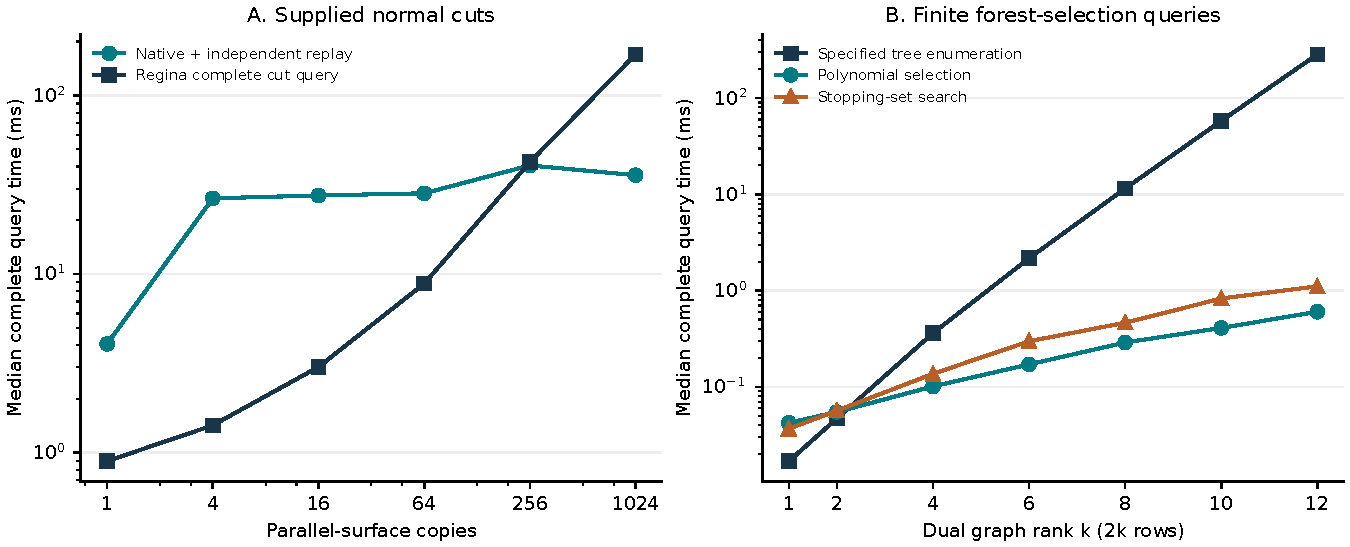
\includegraphics[width=\textwidth]{figures/benchmarks.pdf}
\caption{Recorded complete-query medians.  Left: supplied native cuts,
including independent replay, against the stated Regina route.  Right:
the finite forest-selection family, including the same positive checker
in every arm.  The two panels have different inputs and must not be
combined into a knot-recognition speed-up.}
\label{fig:benchmarks}
\end{figure}

\subsection{Finite decision audit and a controlled enumeration comparison}
The independent finite audit checks 33,995 graph/matrix problems.  Of these,
26,995 are exhaustive enumerations in the stated small families and 7,000
are seeded random cases.  The separate oracle finds 4,554 feasible and
29,441 infeasible instances.  Every general-search certificate replays.
The polynomial solver completes and verifies 23,849 instances; it declines
the other 10,146 because an active column has more than two owners.
These are finite graph/matrix tests, not 33,995 normal-surface examples.

For a controlled comparison, take a chain of $k$ dual links, each replaced
by two parallel edges $a_i,b_i$.  Column $i$ has its sole occurrences on
these two rows, with counts $1$ and $2$, equivalently the capped form of
counts $1$ and $3$.  There are $2^k$ spanning trees.
Every $\{b_i\}$ is a mandatory stopping singleton, so the sole successful
tree is $\{b_1,\ldots,b_k\}$.  The specified include-before-exclude
enumerator, with $a_i$ before $b_i$, reaches this tree last and tests exactly
$2^k$ complete trees.  Stopping search makes $k$ forced choices; the
polynomial solver finds $k$ source-component representatives.  This proves
an exponential separation from that explicit enumeration policy, not a
lower bound against all algorithms.

\begin{table}[htbp]
\centering\small
\caption{Finite forest-selection complete queries, median milliseconds
over five paired rounds.  Every positive arm includes independent replay.}
\label{tab:forest-timing}
\begin{tabular}{rrrrr}
\toprule
$k$ & Trees tested by enumeration & Enumeration & Polynomial & Stopping search\\
\midrule
1 & 2 & 0.0169 & 0.0424 & 0.0368\\
2 & 4 & 0.0470 & 0.0549 & 0.0567\\
4 & 16 & 0.3616 & 0.1012 & 0.1367\\
6 & 64 & 2.1693 & 0.1713 & 0.2978\\
8 & 256 & 11.4927 & 0.2890 & 0.4642\\
10 & 1,024 & 57.8562 & 0.4096 & 0.8278\\
12 & 4,096 & 283.8067 & 0.6030 & 1.1089\\
\bottomrule
\end{tabular}
\end{table}

At $k=12$ the polynomial query is about 470.6 times faster than the
specified enumerator.  At $k=1$ it is about 2.5 times slower.  An identical
enumerator control gives an A/A median-time ratio of 0.987 at $k=12$.
The larger polynomial-only run reaches $k=128$ in 224.3 milliseconds,
including replay.  The hypothetical $2^{128}$ enumeration count there
is a formula, not a measured enumeration run.  Structural visit counters
are included for reproducibility; their totals are not CPU instruction
counts and should not be equated across implementations.

\subsection{Stress tests and remaining measurement limits}
The native focused suite constructs successive interior subdivisions,
exercising up to sixteen interior vertices, as well as normal multiplicity
$2^{4096}$.  It checks a compressed exact census and replay without
enumerating that many normal pieces.  The large-integer case tests the
encoded interface; it does not by itself prove a uniform time bound for
all large-coordinate inputs.  The general finite suite separately tests
huge sparse namespaces and resource exhaustion.

The full repository regression suite passes 1,688 tests in the recorded
run (374.807 seconds).  The standalone finite suite adds 18 focused test
methods; the ten new native methods are included in the 1,688.  The first
sparse checkout lacked historical report fixtures
needed by older tests; those dependencies were restored before the final
regression run.  This setup failure is recorded separately from the final
run and was not counted as a source-code defect or hidden by changing
the tests.  No peak-memory comparison, realistic knot-distribution benchmark,
or end-to-end diagram-recognition timing is claimed in this work.

\section{Toward a quasi-polynomial hierarchy}
\label{sec:research}

\subsection{What this work removes from the complexity budget}
There are three different sizes that must not be conflated: the original
diagram size $n$, the encoded size of a current triangulated or uniform
handle state, and the expanded weight of a normal surface in that state.
The new normalization controls an operation in the second size while
avoiding dependence on the third as a unary parameter.  It does not yet
control how many states are discovered from the first.

In particular, a source with many interior vertices no longer forces an
immediate failure of the finite census method.  Theorem~\ref{thm:native}
removes all its top handles in polynomial encoded time, with no assumption
that their number is logarithmic.  The polynomial selection theorem also
removes a possible enumeration of dual trees in its stated column regime.
For a general matrix, however, the complete selection search retains its
$w^s$ parameter dependence.  The native geometric bound reduces its
original-column difficulty to cycle-compatible triple-unit columns, but
the augmented interface matrix can introduce additional difficulty.

The global composition issue can be stated without hiding an oracle.
Suppose a hierarchy discovery procedure makes at most $Q(n)$ state visits,
including revisits and rejected branches,
every state and emitted certificate has encoded size at most $S(n)$,
and the total discovery, transition-generation, local processing, and replay
work charged to each state visit costs at most $S(n)^d$, for a fixed
constant $d$.  A sequential implementation then costs at most
$Q(n)S(n)^{O(1)}$, plus the explicitly accounted input and output work.
If $Q(n)=2^{O((\log n)^3)}$ and $S(n)=n^{O(1)}$, this is the announced
quasi-polynomial scale.  This elementary composition observation is a
budgeting rule, not a new recognition theorem.

Lackenby's bound $L(g+1)^L$ gives the same scale if a suitable implemented
hierarchy can establish $L=O((\log n)^2)$, $g=n^{O(1)}$, and polynomial
encoded work at every node.  The linear hierarchy bound in the 2026
preprint, by itself, does not imply that logarithmic-square value of $L$
for arbitrary input.  Likewise a theorem that a small certificate exists
does not bound the work of finding it.  These are the principal gaps to
be closed, rather than details that can be suppressed in a local runtime.

\begin{table}[htbp]
\centering\small
\caption{Complexity obligations and their present status.}
\begin{tabular}{>{\raggedright\arraybackslash}p{0.30\textwidth}>{\raggedright\arraybackslash}p{0.60\textwidth}}
\toprule
Obligation & Status in this work\\
\midrule
Compressed cutting & Established in prior literature; the native pipeline
implements a source-certified form.\\
Remove native core three-handles & Proved and implemented in polynomial
encoded time for the admitted source contract.\\
Choose a tree for raw completion & Polynomial in the sparse active-column
case; complete parameterized search in general.\\
Transport recorded bundle ports & Proved and implemented for the current
exposed zero-/one-handle port charts.\\
Transport arbitrary hierarchy patterns & Open implementation and proof
obligation when patterns cross the cancellation support.\\
Find suitable surfaces efficiently & Not solved by this operator;
uniform discovery costs must be bounded.\\
Control state size and hierarchy depth & Must be established relative to
the original diagram, including all resets and certificates.\\
Decide every terminal state & The current raw kernel is sufficient but
incomplete; fourteen corpus cuts remain inconclusive.\\
\bottomrule
\end{tabular}
\end{table}

\subsection{Priority 1: remove the certified interface obstructions}
\paragraph{Question 1: which additional geometric moves discharge the three
saved annular stopping sets?}
The negative packets make this question sharply testable.  On the three
cuts in Table~\ref{tab:interfaces}, altering only the dual spanning tree
cannot work.  A next implementation should keep the authenticated source
and change a precisely named operation: the presentation of a bundle
attachment, a permitted disk-bundle absorption, or a certified lower-handle
move.  It should then show how the formerly nondeletable stopping rows
become removable or disappear under an actual geometric equivalence.
The success criterion is a new replayable genus census, not merely an
algebraic simplification of the row matrix.

\paragraph{Question 2: can an interface obstruction be localized to a
bounded subsurface?}
The saved stopping sets have sizes seven, four, and one.  Trace their
annular curves through the ordered boundary skeleton and determine the
smallest marked subsurface carrying them, together with its complementary
attachment data.  A useful theorem would show that a certified local
replacement has cost polynomial in the subsurface's encoded complexity
and preserves its gluing map relative to the complement.  A graph support
or homology calculation alone cannot guarantee this embedding statement.

\paragraph{Question 3: can primitive but nonunit attaching curves be
recognized with a compressed geometric certificate?}
The ball example shows why unsigned raw counts can stall on a primitive
curve.  One candidate extension is a sequence of boundary isotopies or
slides whose bands are specified by compressed paths and whose effect
on every other ordered attaching curve is independently replayed.
The target is not unrestricted free reduction of a word: cancelling
algebraic inverse letters can conceal geometric intersections with other
bands.  A successful theorem must bound both the move sequence and the
description of the transported curves.  The singleton annular obstruction
is a useful first native test case.

\subsection{Priority 2: solve the remaining native column geometry}
\paragraph{Question 4: is forest-compatible peeling polynomial for
cycle-compatible triple-unit columns?}
Propositions~\ref{prop:three} and~\ref{prop:cycle} show that the original
native columns lie in a much narrower class than general sparse matrices.
The remaining active shape is $(1,1,1)$, and its edges form a triangle,
a parallel pair plus a loop, or three loops.  The question is whether
these geometric restrictions allow an exact extension of the source-SCC
method.  They do not restore matroid exchange, as the explicit counterexample
shows.  An affirmative algorithm therefore needs additional structure;
a negative complexity result would require a reduction that respects
these constraints, preferably with a genuine native realization.

\paragraph{Question 5: is the number of triple-unit columns a useful
parameter?}
Let $k$ count the original columns of shape $(1,1,1)$ after the chosen
lower forest.  A strong target would be an algorithm of cost
$2^{\poly(k)}\poly(m,I)$, or an explicit smaller parameter based on the
interaction graph of those columns.  This would complement the current
$m^{O(s)}$ search when $s$ is large but $k$ is small.  The immediate
combinatorial model consists of ordinary reachability plus two-premise
activation rules.  Treating a two-premise rule as either of its individual
arcs is unsound; both prerequisites must be discharged, and the initial
deletion set must remain a graphic forest.

\paragraph{Question 6: can graphic rank be used earlier inside the
activation process?}
For ordinary source components, disjointness converts all obligations
into a partition matroid.  Ternary activation may create overlapping
obligations.  One approach is to maintain certified disjoint stopping
families and their contracted ranks throughout the search, extracting
short rank defects before branching.  Another is to identify separators
in the joint dual/dependency incidence graph and combine states recording
both connectivity and activation.  The research obligation is an explicit
state-count bound; declaring a separator small without bounding all
boundary partitions does not establish quasi-polynomial complexity.

\paragraph{Question 7: what exactly does changing the lower forest buy?}
The complete search theorem fixes the zero-/one-handle spanning forest.
Changing it changes which cocores survive, and can change the available
raw pivots.  Study paired choices of a lower forest and an upper dual
forest while retaining the source geometric cycles.  A first experiment
should exhaust both choices on the smallest authenticated failures,
record whether success depends on the lower choice, and save a replayable
certificate.  A theorem that bounds a representative family of lower
forests would be more valuable than unrestricted double enumeration.

\subsection{Priority 3: make hierarchy interfaces compositional}
\paragraph{Question 8: can arbitrary marked boundary patterns be transported
through the cancellation balls with bounded encoding growth?}
The present proof fixes exposed native ports.  In a general sutured or
patterned hierarchy, marked curves may cross the support of the selected
top cancellation.  The next geometric compiler must specify how such
curves move across the boundary disk $E$ and the replacement collar,
prove that the cyclic order and essential intersections are preserved,
and bound the growth of the compressed description.  A useful target is
a polynomial bound in the input pattern length and source chart size
per complete forest reduction, rather than a separate expansion at every
three-handle.

\paragraph{Question 9: can support-stratum reuse extend beyond the dual
tree without losing source authentication?}
Corollary~\ref{cor:support} identifies a valid reuse opportunity: the
dual graph and selected tree depend only on zero versus positive source
edge weights.  The full boundary words and bundle multiplicities need
not be constant on that stratum.  Seek a reusable symbolic template for
the retained chart whose variable lengths and endpoint offsets are
explicit arithmetic expressions in normal coordinates.  Each evaluation
must still authenticate the relevant source equalities.  This would
remove repeated structural work while keeping multiplicity-dependent
attachments honest.

\paragraph{Question 10: can local normalization be made confluent at a
useful level of abstraction?}
Different dual trees produce homeomorphic cores with potentially different
raw cancellation success.  Full geometric confluence is therefore too
strong for the present representation.  A more useful target is a canonical
summary of the remaining obstruction class, perhaps in terms of marked
boundary components and a certified family of stopping/rank witnesses.
The summary must preserve the information needed by subsequent cuts;
equal Euler characteristic, equal genus totals, or equal homology alone
does not suffice.

\subsection{Priority 4: close the discovery and global-size gaps}
\paragraph{Question 11: which supplied surfaces can be found with a proved
encoded-time bound?}
Start with a restricted source class where the existence theorem supplies
a normal disk or hierarchy surface of bounded combinatorial type.  Specify
the actual discovery algorithm, the bit lengths of its intermediate
coordinates, and the total unsuccessful work before a certificate is
found.  A normal-coordinate vector supplied by an experiment is an input
to this work's operator, not a discovery algorithm.  A promising bridge
to the hierarchy programme is a certified search over compressed surface
templates whose count can be bounded independently of expanded weight.

\paragraph{Question 12: can one charge every reset to a monotone global
quantity?}
The incoming reports already discuss causal reset budgets and cographic
persistence.  The next step should connect those budgets to the actual
geometric importer and this top normalization.  If an attachment change
invalidates a previous certificate or reintroduces branching, the reset
must have a reason recorded in a global potential.  Seek a statement
bounding the total number and cumulative encoded cost of resets along
every search path.  Independent local size bounds do not prevent an
algorithm from returning to exponentially many distinct states.

\paragraph{Question 13: can the total certificate, including all rejected
branches, be kept quasi-polynomial?}
Positive compressed certificates are often small while a search transcript
is large.  Distinguish a certificate needed to verify the eventual answer
from evidence needed to justify exhaustive failure of a branch.  The
rank defects here illustrate a beneficial compression of negative search.
Identify analogous short obstructions for other hierarchy operations,
and prove that their discovery cost is also controlled.  A concise
negative certificate discovered only after exponential search does not
resolve the runtime question.

\paragraph{Question 14: which terminal procedure should replace raw
cancellation when it is inadequate?}
The present kernel gives useful sufficient certificates, but the geometric
ball example proves its incompleteness in the broader handle category.
An eventual complete hierarchy needs a terminal method with a proved
worst-case budget for every permitted terminal state.  Candidate directions
include restricted geometric simplification, a certified comparison to
standard handlebodies, or a different hierarchy refinement.  The choice
should be evaluated against the actual terminal-state contract rather
than the full unrestricted handlebody problem.

\subsection{Priority 5: verification and credible performance measurement}
\paragraph{Question 15: what is the smallest independent trusted kernel?}
The current replay reduces dependence on discovery code but remains Python
and relies on the existing source geometry checker.  A serious next step
is a written specification for integer decoding, source incidence,
tree reduction, and ordered boundary transport, followed by a small
reference checker or proof-assistant formalization.  The parity constraint
is a useful independently derivable invariant, but should be checked on
uncapped source counts: capping three to two changes parity.

\paragraph{Question 16: where is the practical crossover on nonconstructed
inputs?}
The reported family isolates compression and the finite enumeration
family isolates tree choice.  Neither is a realistic input distribution
for all unknot recognition.  Extend measurement to a stratified native
corpus, reporting triangulation size, coordinate bit length, number of
interior vertices, number of triple-unit columns, interface size, genus
census, certificate size, wall time, and peak memory.  Compare complete
queries with randomized paired order and report regressions.  For an
end-to-end claim, include preprocessing, surface discovery, all rejected
cuts, final certificate production, and replay.

\subsection{Suggested next sequence of work}
The most informative immediate sequence is to resolve the three saved
interface obstructions with a named geometric extension; characterize
cycle-compatible ternary activation on native cores; and implement marked
pattern transport for the resulting reductions.  In parallel, one should
build an accounting layer that records discovery costs and state sizes
against the original diagram.  These tasks turn the current local theorem
and measured coverage improvement into reusable components of a hierarchy
argument.  The general quasi-polynomial recognition theorem remains the
goal to be proved after those obligations are met.

\appendix
\section{Reproducibility, source provenance, and claim ledger}

\subsection{What is in the archive}
The archive contains this PDF and its complete LaTeX source, bibliography,
figure-generation source and rendered figures, a native integration patch,
the proposed native files, the standalone forest solvers and their separate
verifier, focused tests, recorded audit and benchmark output, positive and
negative source packets, and integration/reproduction instructions.
\code{README.md} is the entry point; \code{REPRODUCE.md} gives exact
commands.  \code{code_manifest.json} records the proposed code identities,
and \code{SHA256SUMS.txt} records archive file digests.

The native patch is relative to
\begin{center}\small\basecommit.\end{center}
It is not relative to whichever commit the remote branch later names
\code{main}.  The package's patch validation reconstructs the pinned
original files, applies the patch, and compares the result byte-for-byte
with the supplied proposed files.  A fresh complete clone is preferable
for the full regression suite because older tests import exact reference
implementations and fixtures from historical \code{reports} directories.
Those fixture identities are listed in \code{historical_fixtures.json}
under \code{results/package_validation/}.

The standalone finite tools require only Python's standard library.
The native tests additionally require the pinned ProveIt source tree;
Regina is needed for the comparison audit, not for the replay of the seven
saved positive packets or three source-authenticated negative packets.
Matplotlib is needed only to regenerate the figures.  The article uses
standard pdfLaTeX packages and BibTeX.  Exact commands and recorded versions
are included rather than an implicit environment assumption.

\subsection{Evidence and theorem mapping}
\begin{longtable}{>{\raggedright\arraybackslash}p{0.29\textwidth}>{\raggedright\arraybackslash}p{0.61\textwidth}}
\caption{How each substantive claim is supported.}\label{tab:claims}\\
\toprule
Claim & Proof or independent evidence\\
\midrule\endfirsthead
\toprule Claim & Proof or independent evidence\\\midrule\endhead
Native graph root reachability & Lemma~\ref{lem:rooted}: connected source
one-skeleton with positive edges replaced by root stubs.\\
Geometric reduction of all top handles & Lemma~\ref{lem:dual-cancel} and
Theorem~\ref{thm:native}; actual belt occurrences, not signed coefficients.\\
Retention of native exposed ports & Lemma~\ref{lem:ports}; a relative
boundary-ball argument for authenticated exposed patches.\\
Polynomial encoded graph stage & Bounds on native chart records and
arithmetic in Section~\ref{sec:geometry}; no normal-piece expansion.\\
Stopping characterization & Prior incoming stopping theorem, re-proved
for the stated raw update in Section~\ref{sec:forests}.\\
Complete constrained forest search & Theorem~\ref{thm:search}; independent
branch-covering proof-tree replay.\\
Polynomial sparse-column selection & Reachability and source-SCC lemmas,
Rado's criterion, and a proved shortest-path augmentation.\\
Native total-column bound and parity & Propositions~\ref{prop:three}
and~\ref{prop:cycle}; triangular face regions and the handle-chain identity.\\
85 to 92 complete native cuts & Pinned baseline/native audit, preserved
censuses, 92 independent replays, seven Regina comparisons.\\
Three interface kernels admit no tree & Saved authenticated negative
packets and independent reconstruction of their nondeletable stopping rows.\\
Finite algorithm agreement & 26,995 exhaustive and 7,000 seeded random
oracle comparisons; separate positive and negative checkers.\\
Finite enumeration speed comparison & Specified $2^k$-tree family,
complete-query timings, raw paired rounds and structural counters.\\
Native timing crossover & Six supplied-cut sizes and five randomized
paired rounds per size; scope and regressions retained.\\
General quasi-polynomial unknot recognition & Not proved here.  Discovery,
global-size, pattern-transport, and terminal-completeness obligations remain.\\
\bottomrule
\end{longtable}

\subsection{A small inspectable finite certificate}
The following example is the finite form of the two-choice construction:
\begin{verbatim}
{
  "vertices": 2,
  "columns": 1,
  "edges": [[0, 1], [0, 1]],
  "rows": [[[0, 1]], [[0, 3]]]
}
\end{verbatim}
The tree consists of row 1.  After deleting it, row 0 is removed on
column 0.  A positive finite certificate therefore records the tree
$[1]$ and the peel pair $[0,0]$.  Changing the selected tree to $[0]$
without changing the source fails verification: the surviving count is
three, not one.  If both counts are three, the two stopping singleton
groups have union of graphic rank one, smaller than their group count
two.  That rank defect certifies \code{NO_FOREST}; it does not certify
that the associated manifold is not a ball.

The delivered demonstration generates several such positive and negative
certificates, replays them with the independent checker, and rejects
mutated variants.  The full source packets are larger because they also
authenticate the triangulation, coordinates, geometry, and interfaces.

\subsection{Input validation versus geometric interpretation}
A graph/matrix result can be correct as a finite result even when no
three-manifold realizes the input.  Conversely, a source-authenticated
topological result needs the entire geometric chain of implications.
The manuscript separates these levels to make review practical:
\begin{enumerate}
\item The native source validator establishes the manifold and normal-vector
  contract and authenticates the complementary charts.
\item The geometric dual theorem identifies valid top cancellations and
  the retained native port data.
\item The finite matrix theorem decides exactly the stated raw
  forest-completion problem on those authenticated occurrences.
\item The boundary kernel certifies a genus census when its additional
  attachment criteria succeed.
\end{enumerate}
The last level can remain inconclusive even when the first three succeed.
The ten-core audit demonstrates this distinction directly.  A negative
finite certificate must not cross these levels as a knot verdict.

There is a second distinction between actual counts and saturated counts.
Capping at two is exact for every raw pivot and stopping predicate in
this paper.  It is not exact for parity: an actual count of three is odd
but becomes two.  Proposition~\ref{prop:cycle} uses authenticated uncapped
counts.  The source parity audit follows that convention separately from
the finite solver's capped matrix representation.

\subsection{Attribution and limits of the research claim}
The topological cancellation principle is classical.  Rado's independent
representatives theorem and Edmonds' matroid-intersection framework are
classical.  Compressed normal-surface cutting is established in the
Agol--Hass--Thurston and Lackenby literature.  The stopping-set criterion
and its raw-cancellation extension already occur in the inspected incoming
research.  The contribution claimed here is their specific connection to
the native source geometry, the retained interface proof, the exact
constrained tree-selection formulation and sparse-column solution, the
native column constraints, and the tested certificate implementation.

We did not perform an exhaustive historical priority search for every
combinatorial lemma, and these results have not undergone external peer
review or proof-assistant verification.  The claims are stated so that
they can be checked or refuted independently.  The archive supplies the
counterexamples, exact inputs, patch, raw timings, and negative evidence
needed for that review.  Numerical experiments support implementation
correctness and practical scope; they do not replace the proofs or imply
the unresolved global asymptotic bound.

\clearpage
\phantomsection
\addcontentsline{toc}{section}{References}
\bibliographystyle{plain}
\bibliography{references}
\end{document}
